% RESS Sections 5-8, derived from body.tex (TNNLS version) by P4 R3 script; edit here from now on.
% =====================================================================================================
\section{Experimental protocol}\label{sec:protocol}

\paragraph{Data} The corpus is rebuilt from the raw detections and pixel ground truth of CDnet 2014~\cite{cdnet2014} and
LASIESTA~\cite{lasiesta2016} (frames in true temporal order), with the synthetic part of the BMC benchmark~\cite{bmc2012} as an
off-the-shelf simulator; the detector-defined corpus has \nCorpusT{} events from \nCorpusTvideos{} real videos. For the
twin we use ground-truth events: a frame is a \emph{hit} if a detector box covers at least half of the largest
ground-truth component or overlaps its bounding box with IoU $\ge0.3$, and an event counts if its largest object has at
least 256 pixels (primary definition; the original definition keeps every ground-truth event). Scenes are assigned
to tiers by the category labels of the two datasets. The \emph{static} (main) domain is every CDnet calibration scene
outside the categories \emph{PTZ}, \emph{cameraJitter}, \emph{nightVideos} and \emph{turbulence}, and every LASIESTA
calibration scene outside the categories SM (simulated camera motion) and MC (moving camera): \nMainScenes{} scenes
(\nMainCDnet{} CDnet, \nMainLASIESTA{} LASIESTA; \nDefAllA{} events of any duration, \nMainN{} of at least 32 frames).
The other tiers are night (\nNightScenes{} scenes), turbulence (\nTurbScenes{} scenes; only 2 were run and they hold
\nTurbN{} events, so the tier is reported but not certified) and camera jitter (\nJitterScenes{} scenes: CDnet
\emph{cameraJitter} and LASIESTA SM); the \nPTZScenes{} pan-tilt-zoom and \nMCScenes{} moving-camera scenes are
excluded, because the twin assumes a static background. This definition was fixed after the initial version of this
study, whose static domain was wider; no twin or detector was re-run, and the supplement compares the static domain
of the three versions (Table~S\SuppTabVersions).

\paragraph{Detector and twin} The detector is a fixed single-stage segmentation network (YOLO family~\cite{redmon2016};
yolo26s-seg~\cite{ultralytics}, confidence 0.25, input 640 px, CPU). Per scene, a background plate is the per-pixel median
of up to 60 frames without ground-truth foreground. For each real event and each of three sprite variants (fixed
seeds), the twin removes the real object (mask dilated by 3 px), fills it from the plate, and draws a synthetic object
on the ground-truth trajectory: a vehicle cut from Virtual KITTI~2~\cite{cabon2020vkitti2}, chosen by aspect ratio, or
a procedurally dressed human rendered with MPFB~\cite{mpfb2} with a four-frame walking cycle mirrored to the motion
direction. The sprite height equals the ground-truth box height, its width is clamped to $\pm10\%$ of the box width, its
brightness follows the frame luminance, and a soft shadow is added. Only the object is synthetic; scene, illumination
and background clutter are real. The detector runs on twin frames until the twin hits cover all residues modulo 48,
which is exact for every $K$ dividing 48. The median detector confidence on twin hits is \nConfTwin{} (real:
\nConfReal). Building the twins of the \nMainScenes{} static scenes took \nTwinCostTotal{} CPU-hours (median \nTwinCostScene{} per
scene) on a laptop CPU.

\paragraph{What the twin consumes} The paired twin uses, per camera, empty frames (for the plate) and the annotated
trajectories of the camera's real events (for sprite placement). Calibration therefore costs annotated events:
\nMainN{} at \OPs, i.e.\ \nCalibPerCam{} per static camera when amortized over the domain. For a \emph{new} camera, the
exchange rates below assume that the twin miss rate $q_{\mathrm{new}}$ can be measured without that camera's real
events, e.g.\ with synthetic trajectories drawn on its empty background. We did not build such trajectory-free twins;
we use the paired $q_s$ in their place. The discordance of a trajectory-free twin has not been calibrated, so the
reported savings are conditional on the paired-twin discordance carrying over, and are upper bounds.

\paragraph{Operating points} An operating point is $(\varepsilon,d_{\min},K)$ with events of at least $d_{\min}$
frames. The primary point \OPs{} $=(20\%, 32, 16)$ at $\delta=5\%$ was fixed by a rule chosen before the twin was built
(the largest $K$ for which direct certification needs at most 150 events at 80\% power and the 44 calibration scenes
available at that time give a population bound of at most $\varepsilon/2$), using the pooled real miss rate of all
CDnet events of every category (\nOldPhat{} over \nOldN{} such events, \nOldNreq{} events for direct certification). In the static domain the real miss rate at \OPs{} is only
\nPmainOP; we report this, keep \OPs, and add the sensitivity points OP-A $(20\%,32,8)$ and OP-C $(10\%,32,1)$ and the
full grid $d_{\min}\in\{1,4,8,12,16,24,32\}$, $K\in\{1,2,3,4,6,8,12,16,24,48\}$. The night and turbulence tuning criteria and their held-out
scenes were fixed before tuning. These choices are dated in internal project records but were not publicly registered.
Six choices were made after results were available and are disclosed: (i) the primary event definition (largest
object at least 256 pixels) was adopted after the initial twin run, with the original definition kept as a co-reported
sensitivity (Table~\ref{tab:eventdef}); (ii) the list of LASIESTA calibration scenes, before the split into tiers, was rebuilt (20 to 48 scenes) after correcting
the frame order of that dataset, before the twin was built; (iii) the two held-out turbulence scenes were not run;
(iv) the CDnet \emph{cameraJitter} scenes and (v) the LASIESTA SM and MC scenes were removed from the static domain
after static-domain results were available; and (vi) a second operating point with more real misses was examined after
inspecting the data (Section~\ref{sec:audit}). The operating point \OPs, the audit design and the night criterion were
fixed before the static-domain twin results; everything else in Section~\ref{sec:results} is exploratory.

\paragraph{Why a paired twin} A reweighting alternative~\cite{shimodaira2000} needs overlap between synthetic and real
events. A classifier separating BMC events from real events reaches a median AUC of \nIWtemporal{} with temporal
features, \nIWgeometry{} with geometry and \nIWappearance{} with detector confidence alone (all targets); the gap lies
mostly in geometry, so a reweighted synthetic benchmark cannot stand in for the real event distribution, and the twin
is matched on geometry by construction.

\paragraph{Audit} Leave-one-scene-out (LOSO): each scene is certified with the bound computed from the other scenes.
Monte Carlo (10{,}000 draws): calibration scenes are resampled from the static domain and a new camera is drawn from it;
a false certificate is a certified camera with $p_s>\varepsilon$ (the resampled calibration set may contain the test
camera, which makes this check optimistic; the LOSO audit does not have this defect); the ``truth'' of a camera is its own event pool,
exact over phases. Two must-fail scenarios are run (Section~\ref{sec:audit}). All randomness uses seed 42.

% =====================================================================================================
\section{Results}\label{sec:results}

\subsection{Certificates by tier}
In the static domain, \nMainDw{} of \nMainN{} events at \OPs{} are discordant; hence $\UCP(X,N)=\nMainUfleet$ and,
with $J=\nMainJ$ of \nMainM{} scenes, $\UCP(J,m)=\nMainUpop$ (Table~\ref{tab:tiers}, Fig.~\ref{fig:tiers}). Both are
below $\varepsilon/2=10\%$. In the camera-jitter tier, \nJitDw{} of \nJitN{} events are discordant, all in the CDnet
scene \emph{traffic}, which has real camera shake; the LASIESTA scenes with simulated camera motion have no discordant
event. At
night, \nNightDw{} of \nNightN{} events are discordant (\nNightDwPct; phase-averaged \nNightDexp) and \nNightJ{} of
\nNightScenes{} scenes; pooling all tiers raises the bounds to \nAllUfleet{} and \nAllUpop.

\begin{table}[t]
\centering
\caption{Certificates by tier at \OPs{} ($\delta=5\%$). Discordant events are counted at the worst sampling phase
(in parentheses: phase-averaged count, mean over the three sprite variants; per-scene tables use the majority rule, which
gives \nNightDexpMaj{} at night); $\hat p$, $\hat q$: real and twin miss rates averaged over the phases / at the worst
phase (any fixed deployment phase); $J$ = scenes with a discordant event.}
\label{tab:tiers}
\footnotesize
\setlength{\tabcolsep}{2.5pt}
\begin{tabular}{@{}lrrrrrrr@{}}
\toprule
tier & events & $\hat p$ avg/worst & $\hat q$ avg/worst & discordant & $\UCP(X,N)$ & $J/m$ & $\UCP(J,m)$ \\
\midrule
static (main) & \nMainN & \nPASpMain/\nWPSpMain & \nPASqMain/\nWPSqMain & \nMainDw{} (\nMainDexp) & \nMainUfleet & \nMainJ/\nMainM & \nMainUpop \\
camera jitter & \nJitN & \nPASpJit/\nWPSpJit & \nPASqJit/\nWPSqJit & \nJitDw & \nJitUfleet & \nJitJ/\nJitM & \nJitUpop \\
night & \nNightN & \nPASpNight/\nWPSpNight & \nPASqNight/\nWPSqNight & \nNightDw{} (\nNightDexp) & \nNightUfleet & \nNightJ/\nNightScenes & \nNightUpop \\
turbulence & \nTurbN & \nPASpTurb/\nWPSpTurb & \nPASqTurb/\nWPSqTurb & \nTurbDw & \nTurbUfleet & \nTurbJ/\nTurbM & \nTurbUpop \\
all tiers & \nAllN & \nPASpAll/\nWPSpAll & \nPASqAll/\nWPSqAll & \nAllDw & \nAllUfleet & \nAllJ/\nAllM & \nAllUpop \\
\bottomrule
\end{tabular}
\end{table}

\begin{figure}[t]
\centering
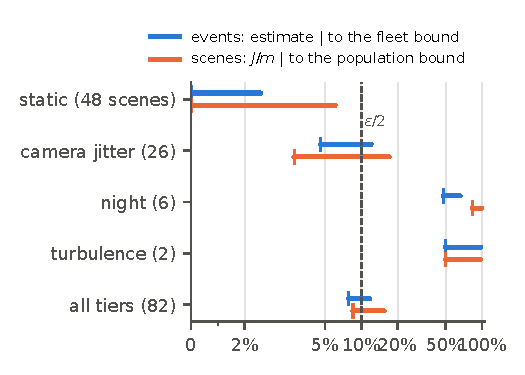
\includegraphics[width=0.8\textwidth]{figs/fig_tiers.pdf}
\caption{Certificates by tier at \OPs{} (event unit, worst phase). Blue: discordant events per event and the fleet bound; orange: discordant scenes per scene and the population bound. Dashed: $\varepsilon/2$.}
\label{fig:tiers}
\end{figure}

\subsection{Exchange rate}\label{sec:exchange}
Fig.~\ref{fig:exchange} and Table~\ref{tab:grid} show the real events a static camera saves when the twin replaces
direct certification, across \nGridPts{} operating points. A camera is certified with no real event when its twin miss
rate plus the transfer bound (both at $\delta/2$, the bound computed without the camera) stays below $\varepsilon$. At
\OPs{} the direct test needs only $n_0=\nNzeroTwenty$ events, because the static-domain miss rate is low; a twin run to
convergence saves those \nSavedOP{} events at \nSavedCamOP{} of \nMainScenes{} cameras, at a measured cost of \nCpuPerSavedOP{}
CPU-hours per saved event (conditional on the discordance carrying over, Section~\ref{sec:protocol}; no accepted camera
has $p_s>\varepsilon$ at \OPs, but acceptances were not audited at every grid cell). \textbf{The twin as built saves no
real events; the saving requires about \nTwinRunsOP{} twin
runs per camera.} With three runs per event, as built, the twin's own miss rate cannot be bounded tightly enough, and at
most \nGridFinMax{} cameras save anything at any grid point. The saving grows with the real miss rate, because direct
certification becomes expensive: it reaches hundreds of events per camera at some grid cells with $\hat p$ above
$10\%$, while at $K=48$ and closer to $\varepsilon$ the twin route saves nothing (Table~\ref{tab:grid}). The target $\varepsilon=20\%$ is a demonstrator, not a safety target. At
$\varepsilon=5\%$ the domain rule requires a population bound of at most $\varepsilon/2=2.5\%$, which needs at least
\nPopScenesQuarter{} calibration scenes even with no discordant scene; with \nMainScenes{} scenes the twin route is not
available at $\varepsilon=5\%$, whatever the twin budget. For the calibrated cameras
themselves, direct Clopper--Pearson on their pooled real misses gives \nDirectPooledU, close to the fleet discordance
bound \nMainUfleet: the fleet certificate adds little where real data exist, and its role is as the building block of
the transfer.

\begin{figure}[t]
\centering
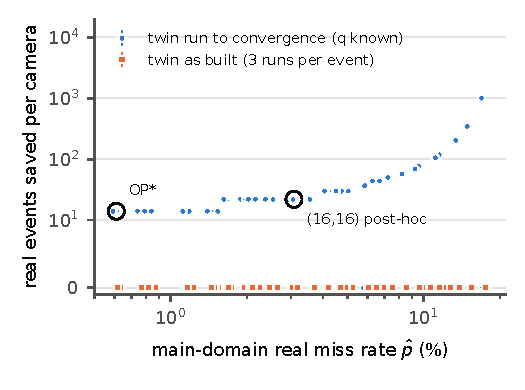
\includegraphics[width=0.8\textwidth]{figs/fig_exchange_rate.pdf}
\caption{Exchange rate: real events saved per static camera (median and interquartile range over \nMainScenes{} cameras) against
the static-domain real miss rate, one point per $(d_{\min},K)$ at $\varepsilon=20\%$. Blue: twin run to convergence;
orange: twin as built (three runs per event). Vertical axis: symmetric log (linear below 10). Circled: \OPs.}
\label{fig:exchange}
\end{figure}

\begin{table}[t]
\centering
\caption{Exchange rate at three operating points (\nMainScenes{} static cameras). $n_{\mathrm{dir}}$: real events of the smallest direct
plan (failures allowed, Clopper--Pearson acceptance) with 80\% power at the pooled static-domain $\hat p$; the
zero-failure plan alone needs $n_0$ events; saved: median real events saved per camera by a twin run to
convergence; runs: twin runs needed per camera; CPU-h: CPU-hours per saved real event.}
\label{tab:exchange}
\setlength{\tabcolsep}{4pt}
\begin{tabular}{@{}lrrrrrr@{}}
\toprule
point & $\hat p$ & $n_{\mathrm{dir}}$ & saved & cams & runs & CPU-h \\
\midrule
\OPs{} $(20\%,32,16)$ & \nTpOPS & \nTndOPS & \nTsvOPS & \nTcamOPS & \nTrunsOPS & \nTcpuOPS \\
OP-A $(20\%,32,8)$ & \nTpOPA & \nTndOPA & \nTsvOPA & \nTcamOPA & \nTrunsOPA & \nTcpuOPA \\
OP-C $(10\%,32,1)$ & \nTpOPC & \nTndOPC & \nTsvOPC & \nTcamOPC & \nTrunsOPC & \nTcpuOPC \\
\midrule
\multicolumn{7}{@{}l}{worst-phase convention (valid for any fixed phase):}\\
\OPs{} & \nWXSp & \nWXSnd & \nWXSsaved & \nWXSacc & \nWXSruns & -- \\
\midrule
\multicolumn{7}{@{}l}{twin as built: cameras saving $=$ \nTcamfinOPS, \nTcamfinOPA, \nTcamfinOPC{} (median saving 0)}\\
\bottomrule
\end{tabular}
\end{table}

\begin{table}[t]
\centering
\caption{Operating-point grid at $\varepsilon=20\%$ (condensed; full grid in the supplement). Each cell: static-domain real miss rate $\hat p$ / real events for direct certification / median real events saved per camera by a twin run to convergence. The twin as built saves none at every cell. OP$^\ast$ is $(32,16)$.}
\label{tab:grid}
\scriptsize
\setlength{\tabcolsep}{3pt}
\begin{tabular}{@{}rccccc@{}}
\toprule
$d_{\min}\backslash K$ & 1 & 8 & 16 & 24 & 48 \\
\midrule
32 & 0.6\%/14/14 & 0.6\%/14/14 & 0.6\%/14/14 & 0.8\%/14/14 & 4.1\%/30/0 \\
24 & 0.6\%/14/14 & 0.7\%/14/14 & 1.2\%/14/14 & 1.6\%/22/22 & 5.8\%/37/0 \\
16 & 1.1\%/14/14 & 1.9\%/22/22 & 3.1\%/22/22 & 4.4\%/30/30 & 9.7\%/76/0 \\
12 & 1.7\%/22/22 & 2.4\%/22/22 & 3.6\%/22/22 & 4.9\%/30/30 & 10.2\%/88/0 \\
8 & 1.6\%/22/22 & 2.9\%/22/22 & 5.0\%/30/30 & 6.7\%/44/44 & 12.2\%/141/0 \\
4 & 2.0\%/22/22 & 6.3\%/44/44 & 9.5\%/76/76 & 11.5\%/118/118 & 17.2\%/1164/0 \\
1 & 2.4\%/22/22 & 11.1\%/106/106 & 14.9\%/348/348 & 16.9\%/1006/1006 & 22.4\%/--/0 \\
\bottomrule
\end{tabular}
\end{table}


\subsection{Audit and must-fail scenarios}\label{sec:audit}
\emph{Is the certificate right because it is empty?} Table~\ref{tab:confusion} cross-tabulates real and twin outcomes.
In the static domain at \OPs{} almost every event is caught by both: \nRealMissEvOP{} events have a real miss at some
phase, in \nRealMissScOP{} scenes, and the twin also misses \nRecallOP{} of the expected real misses, i.e.\ one event.
The zero-discordance result is therefore mostly a statement about a detector that rarely misses in this domain, not a
test of the twin. At night the twin sees almost none of the real misses.

\begin{table}[t]
\centering
\caption{Real versus twin outcomes (expected event counts under a uniform sampling phase; twin = majority of three variants). Recall: share of expected real misses that the twin also misses. \textsuperscript{ph}\,post hoc.}
\label{tab:confusion}
\scriptsize
\setlength{\tabcolsep}{3pt}
\begin{tabular}{@{}lrrr@{}}
\toprule
 & static, OP$^\ast$ & static, $(16,16)$\textsuperscript{ph} & night, OP$^\ast$ \\
\midrule
real miss, twin miss & 1.00 & 4.81 & 0.75 \\
real miss, twin catch ($D$) & 0.31 & 1.94 & 8.31 \\
real catch, twin miss & 0.56 & 3.62 & 0.44 \\
real catch, twin catch & 178.12 & 189.62 & 15.50 \\
\midrule
events & 180 & 200 & 25 \\
events missed at some phase & 4 & 20 & 13 \\
twin recall of real misses & 76\% & 71\% & 8\% \\
\bottomrule
\end{tabular}
\end{table}


\emph{LOSO and Monte Carlo.} At \OPs, the number of static scenes whose discordance exceeds the bound computed
without them is \nLosoOP{} of \nMainScenes{} (Fig.~\ref{fig:loso}); the Monte-Carlo
false-certification rate is \nMcFC. Because real misses are rare at \OPs, this audit cannot reveal much: only
\nScenesPgtEpsOP{} static scene has $p_s>\varepsilon$ there (the one holding the single missed event), and it is refused, so
the 0\% rate rests on that one scene.
A scene above its leave-one-out bound would still be compatible with a population-average guarantee. The informative
tests are must-fail~2 and the camera-jitter check below, which can fail and do.

\emph{Must-fail 1: temporal.} At $K=48$, \nMustFailScenes{} static scenes have $p_s>\varepsilon$ and the procedure refuses
them in \nMustFailRefuse{} of runs; but most of these misses are temporal (events shorter than $K$, which the twin
reproduces by construction); the number of scenes that exceed $\varepsilon$ through detector misses is \nMustFailApp
(Table~\ref{tab:mustfail}, top).

\emph{Must-fail 2: detector.} We add $k$ of the 6 night scenes to the calibration as if they were static-domain scenes;
at \OPs{} every real miss of these scenes is a detector miss. The transfer bound rises with $k$
(Fig.~\ref{fig:leak}, Table~\ref{tab:mustfail}, bottom): from \nLeakUpopZero{} to \nLeakUpopSix{} at \OPs{}, crossing
$\varepsilon/2$ for some subsets at $k=\nLeakWithdrawKfirst$ and for all at $k=\nLeakWithdrawK$, so the domain-level
certificate is withdrawn; no static camera is ever falsely certified (\nMainFCleak). \emph{Out-of-domain pass-through:}
the per-camera rule does not protect the night cameras themselves. The night twin misses almost nothing (its appearance
model only dims the sprite), so each night camera, judged with a bound computed from the static scenes, is certified;
\nNightFC{} of \nNightScenes{} night cameras have $p_s>\varepsilon$ and are falsely certified at \OPs{}
(Table~\ref{tab:mustfail}, middle). Each night miss rate rests on 2 to 10 events and is uncertain; the
finding is that the acceptance rule admitted these cameras although their observed miss rates exceed $\varepsilon$ and
their twins miss almost nothing, not a precise estimate of their miss rates.

\emph{Camera jitter.} The same pass-through occurs for a shaking camera, but it rests on a single scene. Judged by the
twin route calibrated on the static scenes (worst-phase convention, Section~\ref{sec:checks}), \nOODSJitacc{} of the
\nOODSJitcams{} camera-jitter cameras are accepted and \nOODSJitfa{} of them is falsely accepted: \emph{traffic}, a
CDnet scene with real camera shake, whose worst-phase real miss rate is \nOODSJitFApw{} (per-camera table in the
supplement). Its twin catches every event at every phase, because the synthetic object is drawn on a stabilised plate
while the real frames shake; under the phase-averaged reading this camera stays below $\varepsilon$
(Table~\ref{tab:mustfail}, camera-jitter rows), so this failure appears only for a fixed deployment phase. The
LASIESTA scenes with simulated camera motion produce no discordance and no false acceptance, so they add little
evidence either way about real shake. Under the same worst-phase rule \nOODSNightfa{} of
\nOODSNightcams{} night cameras are falsely accepted at \OPs.

\begin{table}[t]
\centering
\caption{Must-fail scenarios. Top: temporal ($d_{\min}=1$, $K=48$), static scenes with $p_s>\varepsilon$, real misses split into detector and temporal misses; all refused in every Monte-Carlo run. Middle: night scenes at OP$^\ast$ (every miss is a detector miss), and whether each is falsely certified when judged alone (phase-averaged); then the same for the camera-jitter scenes. Bottom: population bound when $k$ night scenes leak into the calibration set (median over subsets; withdrawn = share of subsets with a bound above $\varepsilon/2$).}
\label{tab:mustfail}
\scriptsize
\setlength{\tabcolsep}{3pt}
\begin{tabular}{@{}lrrrrrr@{}}
\toprule
\multicolumn{7}{@{}l}{\emph{1: temporal}} \\
scene & $n$ & $p_s$ & detector & temporal & $q_s$ & refused \\
\midrule
port\_0\_17fps & 5 & 99.6\% & 43.3\% & 56.2\% & 100.0\% & 100\% \\
tramCrossroad\_1fps & 11 & 77.7\% & 6.1\% & 71.6\% & 74.2\% & 100\% \\
tunnelExit\_0\_35fps & 34 & 83.6\% & 5.2\% & 78.4\% & 87.9\% & 100\% \\
\midrule
\multicolumn{7}{@{}l}{\emph{2: detector (night)}} \\
scene & $n$ & $p_s$ & $q_s$ & $D_s$ & disc. & false cert. \\
\midrule
bridgeEntry & 2 & 15.6\% & 0.0\% & 15.6\% & 1 & no \\
busyBoulvard & 4 & 96.9\% & 0.0\% & 96.9\% & 4 & yes \\
fluidHighway & 4 & 26.6\% & 0.0\% & 26.6\% & 2 & yes \\
streetCornerAtNight & 10 & 28.1\% & 11.9\% & 20.6\% & 4 & yes \\
tramStation & 2 & 0.0\% & 0.0\% & 0.0\% & 0 & no \\
winterStreet & 3 & 33.3\% & 0.0\% & 33.3\% & 1 & yes \\
\midrule
\multicolumn{7}{@{}l}{\emph{3: detector (camera jitter)}} \\
\midrule
boulevard & 8 & 0.0\% & 0.0\% & 0.0\% & 0 & no \\
traffic & 8 & 3.9\% & 0.0\% & 3.9\% & 3 & no \\
\midrule
$k$ leaked & 0 & 1 & 2 & 3 & 4 & 6 \\
\midrule
$U_{\mathrm{pop}}$ & 3.9\% & 6.0\% & 7.9\% & 8.6\% & 9.4\% & 12.4\% \\
withdrawn & 0\% & 0\% & 0\% & 0\% & 33\% & 100\% \\
\bottomrule
\end{tabular}
\end{table}


\begin{figure}[t]
\centering
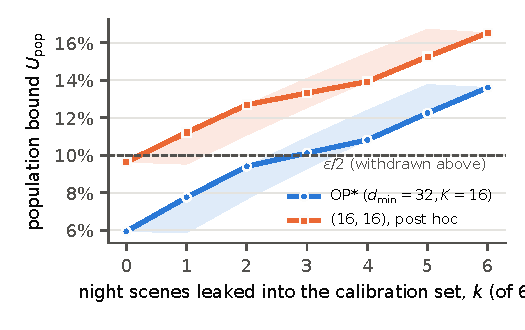
\includegraphics[width=0.8\textwidth]{figs/fig_leak.pdf}
\caption{Must-fail 2: the population bound when $k$ night scenes leak into the static calibration set (median over the
$\binom{6}{k}$ subsets, band: min--max). The domain certificate is withdrawn above $\varepsilon/2$. Individual night
cameras are still certified when judged alone (out-of-domain pass-through, text).}
\label{fig:leak}
\end{figure}

\begin{figure}[t]
\centering
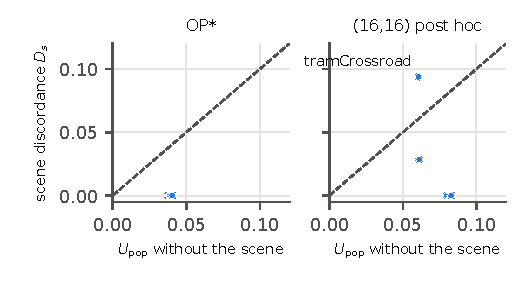
\includegraphics[width=0.8\textwidth]{figs/fig_loso.pdf}
\caption{Leave-one-scene-out: per-scene discordance against the population bound computed without the scene. Points above
the diagonal exceed the bound; the proposition bounds the population mean, not each scene.}
\label{fig:loso}
\end{figure}

\emph{A post-hoc operating point.} To see the certificate under more real misses, the point $(d_{\min},K)=(16,16)$ was
examined after inspecting the data; it fails the criterion we fixed before recomputing it on the static domain (both
bounds at most $\varepsilon/2$ and no false acceptance), because its population bound is \nWPCUpMain, and it is not
reported further.

\subsection{Fixed-phase and site-level checks}\label{sec:checks}
\emph{Worst phase.} A deployed camera keeps one sampling phase. Counting an event as missed if it is missed at any
phase, for the real event, the twin (majority of variants) and the discordance alike, keeps the bound valid for every
fixed phase, because an event missed at some phase is either missed by the twin or discordant at that phase. At \OPs{}
the static-domain real and twin miss rates become \nWPSpMain{} and \nWPSqMain{} (phase-averaged \nPASpMain{} and
\nPASqMain), while the discordance counts and both bounds are unchanged (Table~\ref{tab:tiers}). The direct plan then
needs \nWXSnd{} events, and a twin run to convergence accepts \nWXSacc{} of \nMainScenes{} cameras, saving \nWXSsaved{}
events each (Table~\ref{tab:exchange}); the number of accepted static cameras with a worst-phase real miss rate above
$\varepsilon$ is \nWXSfa.

\emph{Sites.} Scenes filmed at the same site share background, viewpoint and illumination, so the scene may be too fine
a unit of independence. Grouping the static scenes into \nSiteSm{} sites (CDnet challenge categories and LASIESTA
sequence groups, a coarse proxy for sites), the number of sites with a discordant event at \OPs{} is \nSiteSJ, yet
with so few units the population bound is $\UCP(J_{\mathrm{site}},m_{\mathrm{site}})=\nSiteSU$, above $\varepsilon/2$:
under the domain rule the transfer claim is withdrawn at site level. The leave-one-site-out audit finds \nSiteSloso{}
sites above their bound at \OPs. The transfer certificate therefore stands at scene level and is withdrawn at site level; it holds only if
scenes, not sites, are the independent units.

\subsection{Failure modes}
At night the twin sees few real misses: it predicts \nRecallNight{} of the expected missed events, and the tier bound is
\nNightUpop. Fig.~\ref{fig:sprites} shows why: the appearance model scales sprite brightness with the scene, but has no
headlights, glare or sensor noise. An attempt to fix this was specified in advance: night-specific appearance profiles were
tuned on four night scenes and judged on two held-out scenes, with success defined as a median held-out per-scene
discordance of at most 5\%. The best profile barely moved the tuning discordance (\nNightBaseD{} to \nNightProfD,
phase-averaged) and the held-out median was \nNightHeldD{} on \nNightHeldN{} events, so the criterion failed, tuning was
stopped, and night is declared outside the domain. Camera jitter is the second named failure mode, observed in one
scene with real shake: the twin is drawn on a stabilised background plate, so it cannot reproduce the misses caused by
camera shake (over the tier, twin worst-phase miss rate \nWPSqJit{} against a real \nWPSpJit{} at \OPs;
Table~\ref{tab:tiers}). One scene does not show how often real shake produces this failure. The turbulence tier holds
\nTurbN{} events at \OPs{} and is not certified.

\begin{figure}[t]
\centering
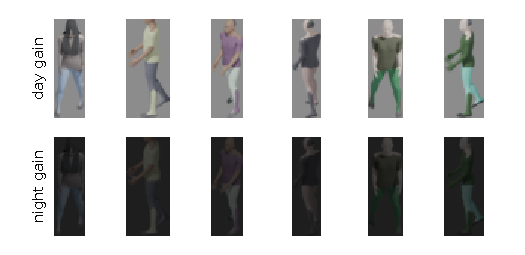
\includegraphics[width=0.8\textwidth]{figs/fig_sprites.pdf}
\caption{Synthetic person sprites (CC0) on a neutral background under the brightness gain used for day and for night
scenes. Dimming alone does not reproduce night imaging, which explains the low twin miss rate at night.}
\label{fig:sprites}
\end{figure}

\subsection{Sensitivity}
\emph{Event definition.} Keeping every ground-truth event (\nDefAllO{} instead of \nDefAllA{} static events of any
duration) leaves \OPs{} almost unchanged: \nOrigN{} events, \nOrigOPDw{} discordant, $\UCP(X,N)=\nOrigOPUfleet$, $J=\nOrigJ$
(Table~\ref{tab:eventdef}).
\emph{Operating point.} At OP-A and OP-C the static-domain miss rate is \nPmainOPA{} and \nPmainOPC{}, and no
static-domain event is discordant.
\emph{Twin details.} The majority rule over sprite variants (1, 2 or 3 of 3) does not change any static-domain count.
Table~\ref{tab:fidelity} compares twin and real hit rates on the same frames: the twin is pessimistic at every
aspect error except one vehicle bin, and both hit rates fall when the ground-truth box has an unusual aspect (occlusion,
objects entering the frame). Clamping the sprite width, which affects \nClampShare{} of twin frames (more than the frames with an aspect error
above 10\% in Table~\ref{tab:fidelity}, because 1-pixel rounding also triggers the clamp), lowers the twin hit
rate by only \nClampExtraDrop{} points more than the real hit rate on the same frames (\nClampPairs{} event--variant
pairs): it inflates $q$, not $D$. The median detector confidence on hits is lower for the twin than for real objects,
especially for persons. Full tables are in the supplement.

\begin{table}[t]
\centering
\caption{Twin fidelity on the same frames (static domain): hit rates by object kind and sprite aspect error before the width clamp, and median detector confidence on hits. Negative differences make the twin pessimistic.}
\label{tab:fidelity}
\scriptsize
\setlength{\tabcolsep}{3pt}
\begin{tabular}{@{}llrrrr@{}}
\toprule
kind & $|$aspect error$|$ & frames & twin hit & real hit & diff.\ (pts) \\
\midrule
person & $\le$10\% & 8,870 & 91.7\% & 94.8\% & -3.2 \\
person & 10-20\% & 5,899 & 90.1\% & 94.2\% & -4.2 \\
person & 20-40\% & 4,404 & 74.0\% & 86.2\% & -12.2 \\
person & $>$40\% & 5,449 & 34.4\% & 44.5\% & -10.0 \\
vehicle & $\le$10\% & 4,105 & 86.9\% & 89.0\% & -2.1 \\
vehicle & 10-20\% & 2,569 & 88.0\% & 90.2\% & -2.2 \\
vehicle & 20-40\% & 3,087 & 87.6\% & 85.1\% & +2.5 \\
vehicle & $>$40\% & 3,881 & 64.9\% & 74.2\% & -9.3 \\
\midrule
person & confidence & & 0.86 & 0.92 & \\
vehicle & confidence & & 0.72 & 0.78 & \\
\bottomrule
\end{tabular}
\end{table}


\begin{table}[t]
\centering
\caption{Event-definition sensitivity (static domain). Primary: largest object $\ge 256$ px; original: every ground-truth event. Discordant events at the worst phase; LOSO: scenes above the bound computed without them.}
\label{tab:eventdef}
\scriptsize
\setlength{\tabcolsep}{3pt}
\begin{tabular}{@{}llrrrrrr@{}}
\toprule
definition & point & $N$ & $\hat p$ & disc. & $\UCP(X,N)$ & $J$ / $\UCP(J,m)$ & LOSO \\
\midrule
primary & OP$^\ast$ & 114 & 0.88\% & 0 & 2.59\% & 0 / 6.1\% & 0 \\
 & OP-A & 114 & 0.88\% & 0 & 2.59\% & 0 / 6.1\% & 0 \\
 & OP-C & 114 & 0.88\% & 0 & 2.59\% & 0 / 6.1\% & 0 \\
\midrule
original & OP$^\ast$ & 116 & 0.86\% & 0 & 2.55\% & 0 / 6.1\% & 0 \\
 & OP-A & 116 & 0.86\% & 0 & 2.55\% & 0 / 6.1\% & 0 \\
 & OP-C & 116 & 0.86\% & 0 & 2.55\% & 0 / 6.1\% & 0 \\
\bottomrule
\end{tabular}
\end{table}


% =====================================================================================================
\section{Discussion and limitations}\label{sec:discussion}

\emph{A narrow window.} Simulation pays in events only when direct certification is expensive, that is, when the real
miss rate is not far below $\varepsilon$; there the twin must also be accurate, and discordances make the transfer bound
grow. When the miss rate is low, $n_0$ is small and there is little to save. The grid (Table~\ref{tab:grid}) shows both
ends: \nNzeroTwenty{} events at \OPs, hundreds at some operating points with $\hat p$ above $10\%$, and nothing
where $\hat p$ comes close to $\varepsilon$.

\emph{Time.} The waiting time saved at camera $s$ is $n_{\mathrm{saved}}/\lambda_s$, where $\lambda_s$ is the event rate
in deployment; we do not estimate it, because the benchmarks publish no frame rates and their clips are dense in events.
If one CPU-hour is valued like one hour of waiting, the twin breaks even when $\lambda_s<1/c\approx\nBreakEven$ events per
hour at \OPs{}, with $c$ the CPU-hours per saved event; this equivalence is an assumption, not a measurement.

\emph{Domain.} The transfer bound is a population-average guarantee: it withdraws the domain certificate when
out-of-domain scenes enter the calibration, but it does not detect an out-of-domain camera. The domain must therefore be
declared and checked by other means (for example, illumination statistics), and a per-camera guarantee requires the
data of Result~4(c). Three items are left for future work: a twin that needs no annotated real trajectory of the new camera, with its own
calibrated discordance; a pre-specified in-domain stress test with cameras whose real miss rate exceeds $\varepsilon$;
and a domain check (for example a per-camera discordance sentinel on a few real events) to stop out-of-domain
pass-through.

\emph{Data and twin.} No static scene has 59 or more qualifying events, so per-camera ground truth is the scene's own
finite event pool; the twin builds its plate from real empty frames and therefore needs a static background; the sprite
library lacks elevated viewpoints for vehicles; and we did not use a full 3-D simulator. The operating point was fixed
from the pooled miss rate of all CDnet events, which turned out to be much higher than the static-domain rate; we kept it
rather than re-select after seeing the twin results. Scenes are not independent draws: several LASIESTA sequences share a room or set-up, and the site-level bound of
Section~\ref{sec:checks} exceeds $\varepsilon/2$. The
cost comparison counts real events and CPU-hours only; annotating the calibration events and building plates are
additional costs. Finally, an event miss is a component-level failure; linking it to a system hazard requires a
hazard analysis of the application.

\emph{Independence and phase.} The results assume independent events given the scene and independent scenes. Events
of one camera share a background, a detector and, in deployment, a single sampling phase; benchmark scenes are not a
random sample of deployments. Correlation of events within a scene does not invalidate the population bound of
Result~4(a) or the leave-one-scene-out audit, because both count scenes, not events: a scene contributes one
indicator whatever the dependence among its events. It does affect the fleet bound of Result~4(b), which counts
events and becomes optimistic under positive within-scene dependence; the population bound needs only independence
across scenes. The main results certify the phase-averaged miss rate; the worst-phase convention of Section~\ref{sec:checks} covers any
fixed phase at a higher real-event cost.

\emph{Threats to validity.} The audit tables and figures use level $\delta$, while acceptance uses $\delta/2$ for the
transfer term; at $\delta/2$ the bounds are larger (Result~4(a)). Software: Python 3.11.9, NumPy 1.26.4, SciPy 1.16.3,
pandas 2.3.3, Ultralytics 8.4.7, OpenCV 4.10.0; CPU: Intel Core i7-1185G7. The detector, the event definition and the
hit rule are fixed; a different detector changes
$p$, $q$ and $D$ but not the theorems. The number of scenes, not the number of events, limits the transfer certificate:
the static domain reaches $\UCP(J,m)=\nMainUpop$ with no discordant scene among \nMainM, and more scenes are needed for
tighter bounds. The audit at \OPs{} is weak because real misses are rare there. The label-based static domain was fixed after the initial version of this
study (Section~\ref{sec:protocol}); its clean audit is therefore partly a result of that post-hoc choice.

\emph{Practical guidance.} The results suggest a simple decision rule for practitioners who consider replacing a
field demonstration with a twin. (i) Compute $n_0$ at the target $(\varepsilon,\delta)$ and estimate the real miss rate;
if it is far below $\varepsilon$, the direct test is already short and a twin can save at most $n_0$ events. (ii) If a
twin is built, declare its domain before calibration and calibrate discordance on as many scenes of that domain as
possible; the number of scenes sets the resolution (Result~4(a)). (iii) Run each new camera's twin long
enough to bound its own miss rate; three runs per event, as here, are not enough. (iv) Do not use the transfer
certificate to admit a camera whose conditions differ from the calibration domain (night, a shaking mount): the
certificate is withdrawn when such scenes enter the calibration, but a single such camera passes through.

\section{Conclusion}\label{sec:conclusion}
Without an assumption linking simulation to reality, synthetic evidence buys no real events in zero-failure
certification, and relaxing the error level buys an exactly computable number. A paired twin turns the question into
one of discordance. The population bound is the transfer guarantee: it counts scenes, tolerates dependence within a
scene, and its price is the number of scenes; the fleet bound covers only the calibrated cameras and assumes independent
events. On the \nMainScenes{} static scenes of this study the transfer certificate stands at scene level
($\UCP(J,m)=\nMainUpop$) but is withdrawn at site level, where \nSiteSm{} sites give \nSiteSU, above $\varepsilon/2$.
Measured on public benchmarks, the exchange rate is modest and domain-bound; at $\varepsilon=5\%$ the transfer needs at
least \nPopScenesQuarter{} calibration scenes. The certificate has two named failure modes, night and camera jitter
(the latter seen in one scene with real shake), in which out-of-domain cameras pass through unless the domain is
declared.
